\section{Datasets Description}
\label{sec:dataset}
Using \platname, we collected full packet traces from Internet activity generated by
mobile devices. We use this data to study how to map monitored traffic to applications, and to
analyze PII leakage. Below, we describe our data-collection methodology, which consists of
1) controlled experiments in a lab setting and 2) IRB-approved ``in the wild'' measurements 
gathered from real users during seven months.

\subsection{Controlled Experiments}
\label{sec:dataset-contr-exper}
Our goal with controlled experiments is 1) to obtain ground truth information 
about network flows generated by apps and devices, and 2) characterize the 
network activity for a large variety of apps in a lab setting. We use 
this data to understand how to model apps' network behavior, how to map network flows 
to the app that generated them and how to identify PII in those network flows. 

\noindent\textbf{Device setup.} We conducted our controlled experiments using three devices: a Galaxy
Nexus running Android 4.2, a Google Nexus running Android 4.0, and
an iPhone 3GS running iOS 6. We start each set of controlled experiments
 with a factory reset of the device to ensure that software installed by previous 
 experiments cannot impact the network traffic generated by each device. 
 Then we connect the device to the
\platname{} platform, we enable the SSL-Bumping plugin, and begin
the experiment. 

\noindent\textbf{Manual tests.} We manually test the
100 most popular free Android apps in the \emph{Google Play} store and 209
iOS applications from the iOS App store on April 4, 2013. For each
application, we install it, enter user credentials for the account if
it is relevant, interact with it for up to 10 minutes, and uninstall
it. This allows us to characterize real user interactions with popular applications 
in a controlled environment. Note that 
because we enter a unique and distinguishable set of user credentials when 
interacting with apps, we can easily extract the corresponding PII from 
network flows (if they are not obfuscated).
\tbd{Do we put the details of apks for malware test here?}

\noindent\textbf{Automated tests.} The second set of controlled experiments consist of fully-automated
experiments on the most popular 732 Android applications from a free,
third-party Android market, \emph{AppsApk.com}~\cite{appsapk}.
We perform this test because Android devices can install
\emph{Third-party applications} that are not available on the
\emph{Google Play} store, without requiring the user to root the device. 

Our goal is to understand how these apps differ from those in the standard \emph{Google Play} 
store, as they are not subject to Google Play restrictions.
\tbd{Is there different constraints on this free market, AR: They do not have paid application. All apps must be free.}
We automate experiments using \emph{adb} to
install each app, connect the device to the \meddle platform, and
start the app. Then we use \emph{Monkey}~\cite{adbmonkey}, an app-scripting 
tool, to perform a series of  approximately100,000 actions that include
random swipes, touches, and text entries.  Finally, we use adb to
uninstall the application and reboot the device to forcibly end any
lingering connections. This set of experiments is limited to
Android devices because iOS does not provide equivalent 
scripting functionality. 

\subsection{In The Wild Measurements}
\label{sec:dataset-wild-measurements}

The controlled experiments in the previous section provide us with 
ground-truth information for a large number of apps running in a controlled 
setting for a short period of time. To understand the network behavior of 
devices with real users "in the wild" over longer time periods, we conducted 
an IRB-approved measurement study with a small set of subjects, from 
Oct. 15, 2012 to Sep. 01, 2013.\footnote{The measurement study is ongoing, we report a subset of results.}

We deployed two \platname servers, one in the USA and one in France
that were used by 26 devices: 10 iPhones, 4 iPads, 1 iPodTouch, and 11
Android phones.  The Android devices in this dataset include the
Nexus, Sony, Samsung, and Gsmart brands while the iPhone devices
include one iPhone~3GS, four iPhone~5, and five iPhone~4S.  These
devices belongs to 21 different users, volunteers for our IRB approved
study.  This dataset, called \mobWild, consists of 318 days with data; the number of 
days for each user varies from 5 to 315 with a median of 35 days.  For privacy reasons, the
SSL-Bumping plugin is \emph{disabled} for all measurements involving
real users.

Capturing all of a subject's Internet traffic raises significant
privacy concerns.  Our IRB-approved study entails informed consent
from subjects who are interviewed in our lab, where the risks and
benefits of our study are clearly explained.  The incentive to use
VPNs is Amazon.com gift certificates awarded by lottery. To protect the
identity of information leaked in the data, we use public key
cryptography to encrypt all data before storing them 
on disk; the private key is
maintained on separate secure severs and with access limited to
approved researchers.  Further, subjects are free to delete their
data and disable monitoring at any time.  Per the terms of our IRB, we cannot 
make this data publicly available due to privacy concerns. We are investigating 
alternative data-collection techniques that provide user anonymity sufficient 
for sharing with other researchers.

\section{Analysis of Mobile Network Flows}

In this section, we analyze the network traces gathered by \meddle to 
1) provide summary statistics of data gathered from our 
users ``in the wild'' and
2) develop and evaluate several techniques for mapping network flows to 
applications, which we will use in subsequent sections to identify privacy 
leaks and malware.

\subsection{Descriptive Statistics from User Study}

This section highlights key features of the dataset gathered from 
users participating in our study (\mobWild). 
Due to the relatively small number of users in our study, we cannot 
draw strong, generalizable conclusions; rather, we use data gathered 
from them to demonstrate that there is a need for \meddle to 
obtain a comprehensive view of Internet traffic from mobile devices. 

\noindent\textbf{Observation 1: \emph{Devices use a variety of networks and use each differently.}} First, we describe the diversity 
of networks that our users connected to. 
We infer the access technology (WiFi or cellular) using the AS description from \emph{WHOIS} data for each IP address used by a mobile device.
Based on this classification, the \mobWild dataset consists of traffic from 65 distinct ASes, of which 8 are cellular ASes and 7 are university networks.
%\tbd{AR: 7 of these ASes belong to Universities -- however if the university is being served by an ISP then I cannot identify it}
During the measurement study, each device connected to our \platname server from at most two distinct cellular ASes. 
In contrast, a median of 4 \wifi ASes were observed per device and for one device we observed traffic from 36 different \wifi ASes spread across 5 countries.
In terms of traffic volumes, collectively our users' who had a cellular data plan for their devices transferred 24-56\% of their traffic over cellular and the remainder over WiFi. 
The key take-away is that, \emph{for our users}, instrumenting a single cellular carrier or WiFi access point misses a 
large fraction of traffic generated by mobile devices. \meddle avoids this limitation.

\noindent\textbf{Observation 2: \emph{Most traffic is HTTP(S), and the dominance of SSL can hinder traffic visibility}.} We use the classification 
provided by Bro~\cite{bro} to categorize flows as either TCP, UDP, or \emph{other}, along with subcategories HTTP, SSL and DNS.
Table~\ref{tab:summaryIOSAndroidTraffic} summarizes the traffic generated by user devices in our study. 

There are two key  
take-aways from this table. First, Web and SSL traffic dominate traffic for users in \mobWild, 
and there is significant diversity in the usage patterns for 
users with Android and iOS devices. For example, 91.26\% (137.63 GB) of the traffic volume in our \mobWild dataset is either HTTP or SSL, 
the fraction of total flows over cellular or \wifi differ significantly for each OS. This motivates the need for a platform that covers 
multiple OSes and multiple access technologies. Second, a significant portion of flows occur over secure (SSL) connections 
that generally prevent classification using deep packet inspection. This calls into question 
the overall effectiveness of traffic optimization approaches that rely 
on middlebox technologies that interpose of plaintext traffic (\eg page rewriting or 
downsampling media). \meddle allows us to avoid this this using SSL bumping.


\begin{table}
\begin{small}
\begin{center}
\begin{tabular}{|p{0.11\columnwidth}|p{0.14\columnwidth}|r|r|r|r|}
\hline
{\bf IP} & \multirow{2}{*}{\bf Service} & \multicolumn{2}{|c|}{\bf Android} & \multicolumn{2}{|c|}{\bf iOS} \tabularnewline
\cline{3-6}
{\bf Protocol} &           &  \textbf{Cell.}  &  \textbf{\wifi}  &  \textbf{Cell.}  &  \textbf{\wifi}  \tabularnewline
\hline
\multirow{3}{*}{TCP}
       &  HTTP (\%)  & 44.83 & 68.23 & 60.07 & 76.92 \tabularnewline
\cline{2-6}
       &  SSL (\%)   & 44.74 & 20.89 & 36.19 & 14.11 \tabularnewline
\cline{2-6}
       &  other (\%) & 8.26  & 10.10  & 2.74  & 1.33 \tabularnewline
\hline
\multirow{2}{*}{UDP}
       &  DNS (\%)   & 1.31  & 0.58  & 0.64  & 0.38  \tabularnewline
\cline{2-6}
       &  other (\%) & 0.54  & 0.11  & 0.31  & 7.24  \tabularnewline
\hline
 Other &  other (\%) & 0.32  & 0.09 & 0.05  & 0.02  \tabularnewline
\hline
\multicolumn{2}{|c|}{\emph{total (\%)}} & 100.00 & 100.00 & 100.00 & 100.00 \tabularnewline
\hline
\multicolumn{2}{|c|}{\emph{Traffic Volume (GB)}}& 9.57 & 21.10 & 16.61  & 103.52 \tabularnewline
\hline
\multicolumn{2}{|c|}{\emph{\# Flows}}   & 927660 & 761735 & 730209 & 2796130 \tabularnewline
\hline
%\multicolumn{2}{|c|}{\emph{\# Devices}} & 10 & 11 & 10 & 15 \tabularnewline
%\hline
\end{tabular}
\end{center}
\end{small}
\caption{\textbf{Traffic volume (in percentage) of popular protocols and services on Android and iOS devices over cellular and \wifi.}
\emph{TCP flows are responsible for more than 90\% of traffic volume. Traffic share of SSL over cellular networks is more than twice the traffic share of SSL over \wifi.}} 
\label{tab:summaryIOSAndroidTraffic}
\end{table}

%An important question for network characterization is which app is responsible for which 
%network flows. As we demonstrate in the following section, previous approaches are insufficient 
%for mapping the majority of apps to their corresponding network flows. We describe 
%several techniques to improve this mapping, and present results for controlled experiments 
%and the \mobWild dataset.

\subsection{Mapping Network Flows to Apps}
%\section{Traffic Classification}
\label{sec:classification-methodology}

Mapping network flows to apps is an important step for determining the origins of potentially costly 
network traffic, and for identifying which apps are responsible for privacy leaks. The following 
sections show that  \emph{previous approaches to classifying passively gathered traffic fail to identify
apps responsible for that traffic most of the time} and that \meddle facilitates a first look at 
determining which apps generate traffic over SSL connections.

%Previous work uses passively gathered data 
%to characterize such traffic, which can be useful for a variety of important topics that include 
%traffic engineering, optimization of network-enabled apps and understanding threats to user privacy. 


% 1) for the users in our study, traffic over WiFi and cellular networks 
%are qualitatively different, and studies that focus on only one technology will miss approximately 
%half of the traffic generated by devices; 

%\subsubsection{Classification of Mobile Apps and Services}

Our \mobWild dataset suggests that apps, OS services and libraries often rely on HTTP and SSL to exchange data~\cite{maier:mobtraffic,falaki:mobileusage,xu:appusage}.
%To analyze the behavior of mobile services we need to first associate the observed flows with the applications and the OS services responsible for the flows.
In the following analysis, we focus on identifying the apps, OS services, and other services responsible for these HTTP and SSL flows. 
We use ground-truth data from controlled experiments to show that the previous approach for classification fails 
for most popular apps; we then develop techniques to improve this mapping and apply it to our \mobWild dataset. 

\subsubsection{Improving HTTP Traffic Classification}

\drc{Update with Ashwin's thesis?}
\tbd{Added text}
Previous works have used these fields in combination with other HTTP header fields to classify and analyze HTTP flows.
However, their focus was to detect misbehaving sources of HTTP traffic such as bots or viruses~\cite{sommers:cellwifi, perdisci:malwaresig, yegneswaran:nemean}, or to identify the category of the apps---gaming, photography,\etc---generating the HTTP flows~\cite{maier:mobtraffic,xu:appusage,falaki:mobileusage,falaki:smartphoneusage}.
Rather that limiting ourselves to category of apps, we now show that the HTTP headers, in particular the \useragent and \httphost fields, can be used to identify the apps and Web services responsible for the HTTP flows.

\begin{table} 
     \centering
     \begin{small}
     \begin{tabular}{|p{0.05\columnwidth}|p{0.08\columnwidth}|p{0.07\columnwidth}|p{0.08\columnwidth}|p{0.09\columnwidth}|p{0.09\columnwidth}|p{0.09\columnwidth}|p{0.09\columnwidth}|}
        \hline
        {\bf OS}&{\bf Store}&{\bf Apps}&{\bf Gen.}&\multicolumn{2}{|c|}{\bf Host} & {\bf User-}&{\bf Combi-} \tabularnewline
        \cline{5-6}    
             &        &     & {\bf HTTP} & {\bf App. } & {\bf Org.}& \bf{Agent}   & \bf{nation}  \tabularnewline                
        \hline    
        iOS  & Apple  & 209 & 176 & 83 (47.1\%)  &  119 (67.6\%)   &  149 (84.6\%)& 157 (89.2\%) \tabularnewline
        \hline
        And. & Google & 100 & 92  & 41 (44.5\%)  &  54 (58.6\%)    &  21 (22.8\%) &  59 (64.1\%)  \tabularnewline
        \hline    
        And. & Other  & 732 &  365 &  17 (4.6\%) &  79 (21.6\%)    &  52 (14.2\%)  & 83 (22.7\%)  \tabularnewline
        \hline
     \end{tabular}
     \end{small}
     \caption{\textbf{Classification of apps based on \httphost and \useragent.} \emph{ A large majority of iOS apps use dedicated \useragent strings to fetch data over HTTP. A combination of \useragent and \httphost can be used to identify the majority of Android and iOS apps.}}
     \label{tab:classification-success}
\vspace{\postfigspace}
\end{table}

%%
%% No HTTP Traffic from 209 - 38 = 171; 171 + 5 (OS possibly - confirm) = 176  ,
%% 181 unique signature, 7*2 = 14 duplicate (fooducate, fdct). 
%% 174 unique application signatures found
%% 5 UA belonged to OS services, geoservices, applecoremedia, gamedkit, securityd, mmsdk 
%% Ads from 98 - 4 -> 94 labels
%% Rough estimate of HTTP for apps because mapping  -- 414 files without HTTP
%%%
%% In amy dataset, 
%% 132 generate only ad traffic 


\noindent\textbf{Controlled experiments.}
In Table~\ref{tab:classification-success} we present results from our classification study using controlled experiments. To 
the best of our knowledge, we are the first to attempt to use ground-truth information to evaluate the 
effectiveness of app classification using only header data.

\emph{iOS:}
First, we note that 176 of the 209 iOS apps we manually tested generated HTTP traffic.
We observe that the \httphost field uniquely identified the corresponding app for 47\% of the iOS apps we tested (column 5); the flows containing the application signature was responsible from 15\% to 98\% of the traffic volume from the application during  our measurements. The rest of the traffic was either due to ads or to CDNs that did not contain the app signature.  
The \httphost field also can identify the provider that released an app (\eg Zynga but not \emph{Farmville}).
In column 6 of Table~\ref{tab:classification-success}, we see that classification by organization is effective for 67\% of iOS apps. 

\emph{Android:} We observe similar results for flows from apps in Google Play.
However, for the apps from the Third-party store we observe that the \httphost field is less effective. 
Primarily this is due to the fact that a majority of the apps we tested (about 77\%) were stand-alone services such as games where the provider did not use its own Web service. 
Instead, these apps either contacted some advertisement sites or sites hosted by CDNs. 
While we can use the \httphost field to identify these 3rd-party sites contacted by an app, we cannot determine which app generated the traffic. 

\emph{Augmenting with \useragent: } We now show that by augmenting the information in the \useragent to the information gained by the \httphost field, we can classify a majority of iOS and Android apps. 
In our controlled experiments we observed a non-empty \useragent string in more than 99.7\% of the HTTP flows from iOS and 90.9\%flows from Android. 

A \useragent string may contain an app identifier and other auxiliary information such as details of the OS, manufacturer, and compatibility with Web browsers~\cite{mozilla:useragentdetection}. 
For example, Yahoo Mail's \useragent string contains the string \emph{YahooMobileMail/1.0}. 
However, some apps use more generic \useragent strings such as \emph{AppleCoreMedia} (streaming video on iOS) or \emph{Dalvik} (generic text for Android). 
To extract the app information, we use a set of regular expressions to filter out the auxiliary information in the \useragent and further cluster these extracted tokens using the edit distance between the tokens.

Table~\ref{tab:classification-success} shows that 84.6\% of the 176 iOS apps generating HTTP traffic were correctly identified based \useragent, which we verified by manual inspection.
However, this works only for 23\% of the Android apps generating HTTP traffic. 
For the 27 iOS apps which we failed to identify, we observed signatures for OS services and libraries.
% such as \emph{Apple Core Media}, \emph{Game Kit}, \emph{Geo Services}, etc. and signatures of third-party libraries and services such as \emph{Google Analytics} and \emph{Adobe Air}.
Similarly, the majority of Android HTTP traffic contained flows with the default \useragent (\emph{Dalvik}).
%Further, for the apps from the third-party store, we observe that the \useragent for ads and analytics libraries such as \emph{Google Analytics} and \emph{Adsense for Mobile} were the most common \useragent after the default \useragent.

To summarize, \useragent is more effective for classifying iOS apps and \httphost is more effective for Android apps; however, neither alone is a complete solution. 
To fill this gap, we are currently investigating how to use ad-network identifiers to classify apps. 

\begin{figure}
\subfloat[iOS]{\label{fig:http-wordcloud-ios}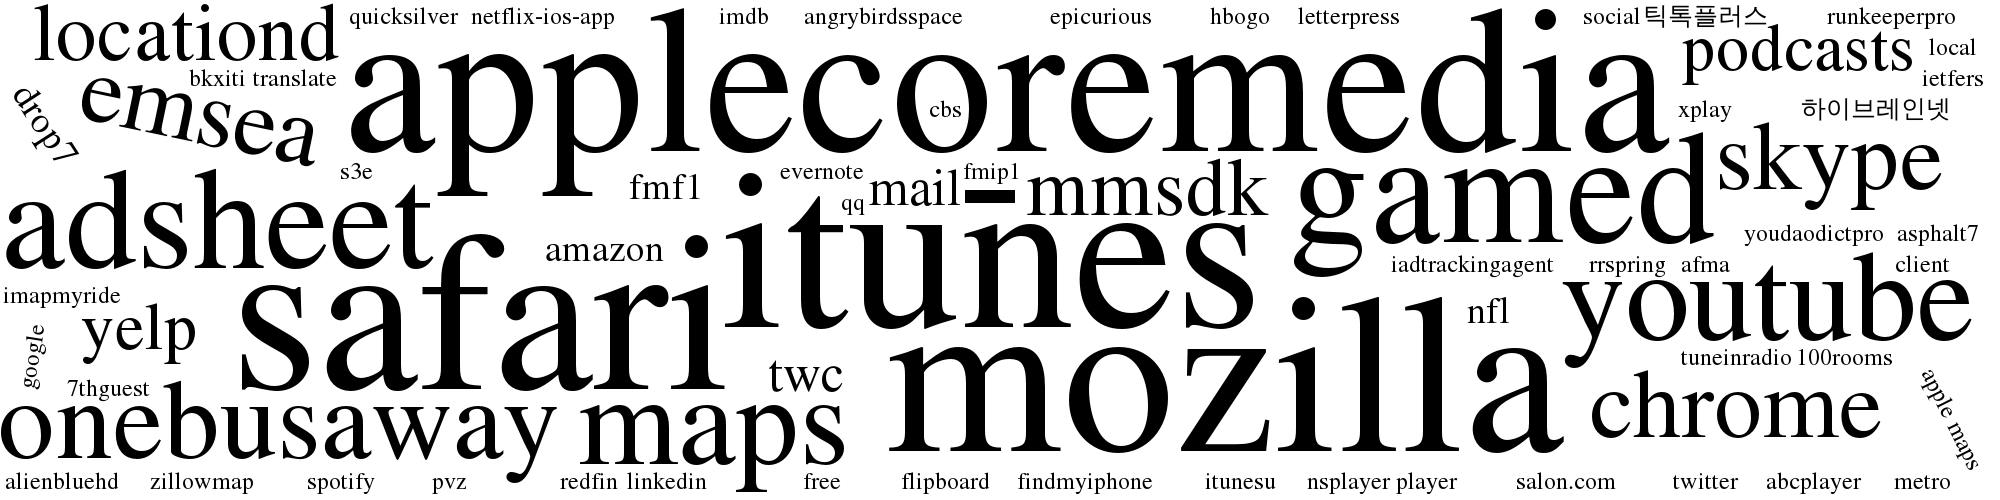
\includegraphics[width=\columnwidth]{figures/wordcloud_useragentsignature_ios_image.png}}\newline
\subfloat[Android]{\label{fig:http-wordcloud-android}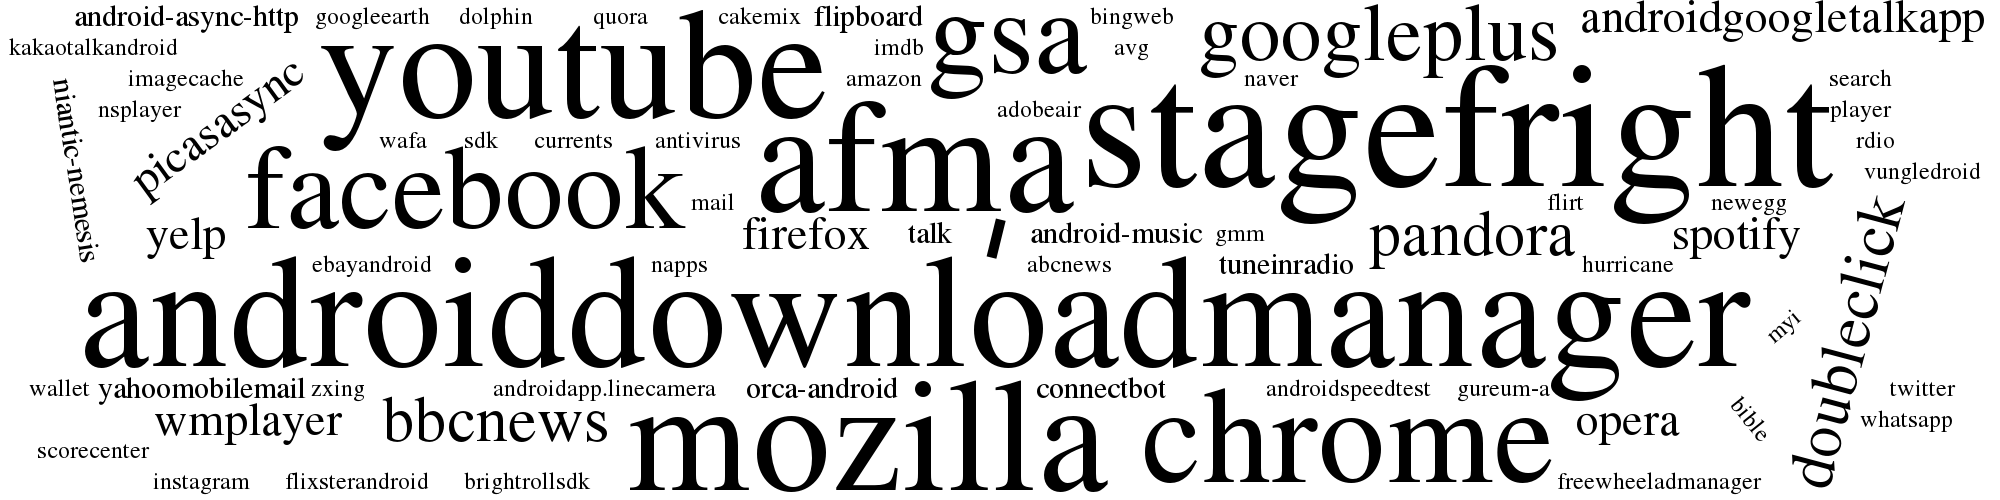
\includegraphics[width=\columnwidth]{figures/wordcloud_useragentsignature_android_image.png}}
\caption{\textbf{\useragent signatures in  iOS and Android HTTP flows.} \emph{The font weight represents the number of users for which a particular signature was observed.}}
\vspace{\postfigspace}
\label{fig:http-wordcloud}
\end{figure}

\textbf{In the wild data.}
We now describe the results of our classification on data gathered from our user study.
Using only the \useragent on the \mobWild dataset we were able to map flows to 256 iOS and 86 Android apps, OS libraries, and services. 
The \emph{word cloud} in Fig.~\ref{fig:http-wordcloud} contains the summary of our results; the font size of a signature is proportional to the number of users for which the signature was observed.
Note that \emph{Apple Core Media} and \emph{Stagefright} are services for downloading media content on iOS and Android devices, respectively.
For the iOS devices in the \mobWild dataset, we observe a signature of \emph{Apple Core Media} in more than 98.45\% of the content downloaded from the YouTube servers (identified by their \httphost field).
Similarly, depending the Android version we observe either the signature for Stagefright or no app or OS service signature for YouTube traffic. % to Android devices depending on the OS version. 
We observe a similar signatures for other popular media services such as Netflix, YouTube, Vimeo, Pandora, etc, so we use the \httphost field to identify these Web services.


\begin{table}
\centering
\begin{small}
\begin{tabular}{|p{0.15\columnwidth}|p{0.2\columnwidth}|c|c|c|c|}
\hline
\multirow{2}{*}{\bf Technique}&\multirow{2}{*}{\bf Category} & \multicolumn{2}{c|}{\bf iOS} &  \multicolumn{2}{c|}{\bf Android} \tabularnewline
\cline{3-6}
&   & {\bf Bytes}  & {\bf Flows} & {\bf Bytes} & {\bf Flows}   \tabularnewline
&   & {\bf (\%)}  & {\bf (\%)} & {\bf (\%)} & {\bf (\%)}   \tabularnewline

\hline
\multirow{2}{*}{\useragent} &Apps             & 43.21  & 85.73 & 15.01 & 75.17 \tabularnewline
\cline{2-6}
                            & OS Services$^{*}$            &  0.19  & 3.82 & 17.42 & 0.81 \tabularnewline
\hline
\useragent + &Media (Popular)         & 51.36  & 7.12  & 61.98 & 3.56 \tabularnewline
\cline{2-6}
\httphost  &Media (Other)           & 4.90  &  0.85 &  0.68 &  0.12 \tabularnewline
\hline
\httphost & Other Apps/Web-services  & $<$0.01 & 0.49 & 1.53  & 12.98 \tabularnewline
\hline
\multicolumn{2}{|c|}{Total Classified}  & {\bf 99.6} & {\bf 98.01} & {\bf 96.62} & {\bf 92.64} \tabularnewline
\hline
\end{tabular}
\end{small}
\caption{\textbf{Classification of HTTP Traffic}. \emph{OS services$^{*}$ includes services other than those used to download media content.}}
\label{tab:classify-http}
\end{table}


In Table~\ref{tab:classify-http}, we observe that with a combination of \useragent and \httphost field in HTTP headers, we were able to classify more than 92\% of the traffic in terms of flows and bytes from iOS and Android devices.
We observe that media from popular hosts in our \mobWild dataset, including Netflix, YouTube, Pandora, Spotify, and Vimeo, contribute to more than 50\% of the traffic volume from iOS and Android devices.
We also observe that media served from CDNs and others hosts from which we could not identify the Web service from other fields in the HTTP header, comprises less than 5\% of the traffic volume for the iOS and Android devices in our dataset.

\subsubsection{SSL Traffic Classification without Decryption}

SSL flows provide limited information in plaintext that identify apps. 
For the traces captured during our controlled experiments, we use SSL bumping to classify HTTP flows using 
the techniques described in the previous section. 
However, we did not perform SSL bumping for the devices in the \mobWild dataset, so we now describe how to 
classify SSL flows \emph{without decryption}. 

\noindent\textbf{Overview of Classification technique.}
Using port numbers, we observe in that more than 99\% of the SSL flows observed in our controlled experiments were due to HTTPS, the rest of the flows were due to email, instant messaging, and OS notification services. 
We therefore focus our attention on identifying the Web services responsible for the HTTPS flows.
We use the DNS messages and subsequent SSL handshakes to determine the \emph{hostnames} of the remote hosts contacted by mobile devices.
We then map these hostnames to Web services using our technique for HTTP traffic classification.

Once we identify the hostnames, we classify the traffic in two phases.
In the first phase we use the port number and hostname to identify the service and group the traffic based on service.
The five most popular groups that we found in our dataset are social network, mail, media, instant messages, and notification.
For example, flows to \emph{facebook.com}, \emph{twitter.com}, \emph{plus.google.com} are grouped as social networks.
Traffic to well known email ports such as TCP port 993, and traffic to hosts such as \emph{mail.google.com} are classified as mail traffic.
Similarly, we use documented ports to identify notification services (Android push) and instant messages (Facebook Messenger).

In the second phase, we group hostnames that do not contain details of Web services.
For example, the hostname \emph{fbcdn-photos-a.akamaihd.net} is a strong indication that the traffic is due to Facebook (due to \emph{fbcdn}), while \emph{www.googleapis.com} hides the underlying app and Web services.
We group hostnames that hide the app and Web service based on the parent organization.
During manual examination of the traces, we observe two main groups: Google Services and Apple Services.
Google Services includes flows whose remote hosts are served by Google, for example, \emph{www.googleapis.com}, while Apple Services includes flows to servers managed by Apple, for example, \emph{*.phobos.apple.com}
This classification, though crude, gives insights on the key sources of SSL traffic.

\noindent\textbf{Identifying Hostnames using SSL Handshake.}
We first use the common name (CN) field of certificates to identify the servers that exchanged data using HTTPS.
We observe that less than 25\% of the HTTPS traffic from iOS and Android contains the fully qualified domain name (FQDN) in the subject of the certificate; the rest of the traffic either contains regular expressions such as *.google.com in the certificate or is a continuation of a previous SSL session. 
To further resolve the hostnames, we rely on \emph{Server Name Indication} (SNI) used by SSL flows~\cite{rfc:servernametls}.
Servers that host multiple services use the SNI to distinguish these services.   
For example, we observe an SNI of \emph{plus.google.com} and \emph{s.youtube.com} in two flows that used a certificate with a CN \emph{*.google.com}.
Using either the certificate or the SNI we were able to identify the name of the Web service in less than 40\% of HTTPS traffic.

\noindent\textbf{DNS mapping.} 
For the remaining flows we use DNS requests made by the mobile devices before starting the HTTPS flows, a technique similar to DN-Hunter~\cite{bermudez:dnhunter}.
DN-Hunter relies on the most recent FQDN that corresponds to the IP address, however in our controlled experiments we observe Android and iOS devices use the first entry in DNS response while resolving \emph{hostnames}.
We therefore use the latest DNS response that contains the IP address of the Web service in the first position.
In spite of the potential usefulness of DNS responses, we give a high priority to the server-name and the certificates because the DNS response differs from these in 9.2\% of the iOS traffic and 5.6\% of Android traffic.
This difference is either due to caching of DNS requests or when the same IP is used for multiple services. 

\begin{table}
\centering
\begin{small}
\begin{tabular}{|p{0.1\columnwidth}|p{0.2\columnwidth}|c|c|c|c|}
\hline
\multirow{2}{*}{\bf Phase} & \multirow{2}{*}{\bf Category} & \multicolumn{2}{c|}{\bf iOS Traffic} &  \multicolumn{2}{c|}{\bf Android Traffic} \tabularnewline
\cline{3-6}
 &         & {\bf Bytes}  & {\bf Flows} & {\bf Bytes} & {\bf Flows}   \tabularnewline
 &         & {\bf (\%)}  & {\bf (\%)} & {\bf (\%)} & {\bf (\%)}   \tabularnewline
\hline
\multirow{5}{*}{Phase 1}
& Social Networks    & 12.81 &  7.74 & 35.39 & 19.28 \tabularnewline
\cline{2-6}
& Mail               &  6.11 &  9.26 &  6.46 & 11.02 \tabularnewline
\cline{2-6}
& Media              &  0.94 &  0.25 &  3.66 &  3.62 \tabularnewline
\cline{2-6}
& Instant Messages   &  3.70 & 14.09 &  0.21 &  0.48 \tabularnewline
\cline{2-6}
& Notifications     &  4.69 & 17.45 &  2.02 &  6.57 \tabularnewline
\cline{2-6}
%\hline
& \emph{Total (A) }       & {\em 28.25} & {\em 48.79} & {\em 47.74} & {\em 40.97} \tabularnewline
\hline
\multirow{2}{*}{Phase 2}
 & Google Services   & 36.32 & 17.56 & 47.31 & 48.27 \tabularnewline
\cline{2-6}
 & Apple Services    & 25.26 & 28.26 & $<$0.01 & $<$0.01 \tabularnewline
\cline{2-6}
& \emph{Total (B) }       & {\em 61.58} & {\em 45.82} & {\em 47.31} & {\em 48.27} \tabularnewline
\hline
\multicolumn{2}{|c|}{\emph{Total (A + B)}}       & {\em 89.83} & {\em 94.61} & {\em 96.10}  &  {\em 89.24} \tabularnewline
\hline
\end{tabular}
\end{small}
\caption{\textbf{Classification of SSL traffic in the \mobWild dataset.} \emph{The iOS and Android SSL traffic in the \mobWild dataset is dominated by Google and Apple Services. The share of Social Network traffic is higher for Android devices because the default photo backup services on Android devices uses the Google Plus (and Picasa) Social Network.}}
\label{tab:classify-ssl-traffic}
\end{table}

\noindent\textbf{Classification results.} 
Table~\ref{tab:classify-ssl-traffic} shows our SSL classification results on the SSL traffic in the \mobWild dataset. 
As discussed previously, we first group hostnames depending on the type of app and Web service.
For flows whose hostnames are ambiguous, we group them according to organizations such as Google and Apple.

In Table~\ref{tab:classify-ssl-traffic}, we observe that 61.5\% of iOS and 47.3\% of Android traffic (by bytes) is respectively to Google and Apple servers where the hostname does not contain signatures of the App and Web service.
This share does not include the traffic to Google and Apple servers that we classified as Social Network, Instant Messaging, Mail, and Media.
For example, the share of Social Network traffic is higher for Android devices compared to iOS devices because the default photo backup services on Android devices uses the Google Plus (and Picasa) Social Network.
Google services and Apple services are therefore the largest sources of SSL traffic in our \mobWild dataset.

In summary, using the certificates, SNI, and DNS messages, we were able to identify the hostname of the remote hosts for more than 90\% of the SSL flows.
These hostnames contain signatures of the Web services and Apps responsible for these SSL flows.
We observe that Google and Apple are the dominant sources of SSL traffic in both datasets.

\subsubsection{Summary}

Our goal was to identify the apps and Web services responsible for the network traffic flowing through \meddle servers.
To meet this goal we used results from our controlled experiments to obtain the ground truth information on network flows generated by apps and OS services.
We then use the a combination of \useragent and \httphost field to identify apps and Web services responsible for HTTP flows.
Similarly, we use certificates, SNI, and DNS messages to classify SSL flows.
In the following sections, we will use this classification to identify and block privacy leaks and malware.

%%% Local Variables: 
%%% mode: latex
%%% TeX-master: "main"
%%% End: 


